\section*{Problem Set 7 Due 11am, Monday, May 4, 2026}

\question{1}{\textbf{Comparing Z-boson partial widths}}\\
For massless fermions, the tree-level decay width of the $Z$ boson is
\begin{align}
    \Gamma(Z \to f \bar{f}) = N_f^c \frac{G_F M_Z^3}{6\sqrt{2}\pi} \left((g_V^f)^2 + (g_A^f)^2\right),
\end{align}
where $N_f^c=1$ for leptons and $N_f^c=3$ for quarks, and 
\begin{align}
    g_V^f = T_3^f - 2 Q_f \sin^2\theta_W, \quad g_A^f = T_3^f.
\end{align}
Take $\sin^2\theta_W = 0.231$, and neglect fermion masses and radiative corrections.

\begin{itemize}
    \item [(a)] For $f=\nu, e, u, d, b$, list $T_3^f$, and $Q_f$, and compute $g_V^f$, $g_A^f$, and $(g_V^f)^2 + (g_A^f)^2$.
    \item [(b)] Rank the partial widths 
    \begin{align}
        \Gamma(Z \to \nu \bar{\nu}), \quad \Gamma(Z \to e^+ e^-), \quad \Gamma(Z \to u \bar{u}), \quad \Gamma(Z \to d \bar{d}), \quad \Gamma(Z \to b \bar{b})
    \end{align}
    from largest to smallest, indicating any equalities.
    \item [(c)] Briefly explain your ranking. In particular, explain why $\Gamma(Z \to e^+ e^-)$ is smaller than $\Gamma(Z \to \nu \bar{\nu})$, and why quark final states make the dominant contribution to the total $Z$ width.
\end{itemize}

\answer{}
\begin{itemize}
    \item [(a)]
\end{itemize}
The values of $T_3^f$, $Q_f$, $g_V^f$, $g_A^f$, and $(g_V^f)^2 + (g_A^f)^2$ for $f=\nu, e, u, d, b$ are listed in Table \ref{HW7:table: Quantum numbers and couplings}.
\begin{table}[h!]
\centering
\begin{tabular}{|c| c | c|  c|  c | c |} 
    \hline
    $f$ & $T_3^f$ & $Q_f$  & $g_V^f=T_3^f - 2 Q_f \sin^2\theta_W$ & $g_A^f=T_3^f$  & $(g_V^f)^2 + (g_A^f)^2$ \\
    \hline
    $\nu$ & $+1/2$ & $0$ & $+1/2$ &$+1/2$ &$0.5000$ \\
    $e$ & $-1/2$ & $-1$ & $-1/2+2\sin^2\theta_W=-0.038$ & $-1/2$&  $0.2514$\\
    $u$ & $+1/2$ & $2/3$ & $+1/2-4/3\sin^2\theta_W=0.192$ & $+1/2$&  $0.2868$ \\
    $d$ & $-1/2$ & $-1/3$ & $-1/2+2/3\sin^2\theta_W=-0.346$ & $-1/2$&  $0.3697$ \\
    $b$ & $-1/2$ & $-1/3$ & $-1/2+2/3\sin^2\theta_W=-0.346$ & $-1/2$&  $0.3697$ \\
    \hline
\end{tabular}
\caption{ Values of $T_3^f$, $Q_f$, $g_V^f$, $g_A^f$, and $(g_V^f)^2 + (g_A^f)^2$ for $f=\nu, e, u, d, b$.}
\label{HW7:table: Quantum numbers and couplings}
\end{table}

\begin{itemize}
    \item [(b)]
\end{itemize}
Since the partial width is proportional to $N_f^c ((g_V^f)^2 + (g_A^f)^2)$, we have
\begin{align}
    \Gamma(Z\to\nu\bar{\nu}) &\propto 1 \times 0.5000 = 0.5000, \\
    \Gamma(Z\to e^+ e^-) &\propto 1 \times 0.2514 = 0.2514, \\
    \Gamma(Z\to u \bar{u}) &\propto 3 \times 0.2868 = 0.8604, \\
    \Gamma(Z\to d \bar{d}) &\propto 3 \times 0.3697 = 1.1091, \\
    \Gamma(Z\to b \bar{b}) &\propto 3 \times 0.3697 = 1.1091.
\end{align}
Thus, the ranking from largest to smallest is
\begin{align}
    \Gamma(Z\to d \bar{d}) \approx \Gamma(Z\to b \bar{b}) > \Gamma(Z\to u \bar{u}) > \Gamma(Z\to \nu \bar{\nu}) > \Gamma(Z\to e^+ e^-).
\end{align}

\textbf{Note:} Of couurse, we can include other quark flavors ($s, c$) in the ranking as well. Then the ranking from largest to smallest is 
\begin{align}
    \Gamma(Z\to d \bar{d}) \approx \Gamma(Z\to s \bar{s}) \approx \Gamma(Z\to b \bar{b}) > \Gamma(Z\to u \bar{u}) \approx \Gamma(Z\to c \bar{c}) > \Gamma(Z\to \nu \bar{\nu}) > \Gamma(Z\to e^+ e^-).
\end{align}

Here, we ignore the mass differences between the quark flavors, which is a good approximation for $u, d, s$ quarks, but not a good approximation for $c, b$ quarks. Also, we ignore the loop-level corrections to the $Z$. 


\begin{itemize}
    \item [(c)]
\end{itemize}
The partial width $\Gamma(Z\to e^+ e^-)$ is smaller than $\Gamma(Z\to \nu \bar{\nu})$ because the vector coupling $g_V^e$ is suppressed by the factor $1-4\sin^2\theta_W \approx 0.076$, which is close to zero, while $g_V^\nu$ is not suppressed. 

Besides, because of the color factor $N_f^c=3$ for quarks, which enhances the partial widths for quark final states compared to leptonic final states, quark final states make the dominant contribution to the total $Z$ width. Including all possible quark flavors ($u, d, s, c, b$) further increases the total width from quark final states, making it even more dominant compared to leptonic final states.\qed







\clearpage
\question{2}{\textbf{Higgs potential with a higher-dimension correction}}\\
The Standard Model Higgs potential can be modified by higher-dimension operators that parameterize possible effects of heavy new physics. As a simple example, consider 
\begin{align}
    V(H)= -\mu^2 H^\dagger H + \lambda (H^\dagger H)^2 + \frac{c_6}{\Lambda^2} (H^\dagger H)^3,
\end{align}
where $\mu^2>0$, $\lambda>0$, and $c_6$ is a dimensionless coupling, and $\Lambda$ is a heavy mass scale. Assume this is the only relevant higher-dimension correction to the Higgs potential. Work in unitary gauge 
\begin{align}
    H= \frac{1}{\sqrt{2}} \begin{pmatrix} 0 \\ v+h \end{pmatrix}.
\end{align}

\begin{itemize}
    \item [(a)] Derive the condition that determines the vacuum expectation value $v$ by minimizing the potential.
    \item [(b)] Expand the potential to quadratic and cubic order in $h$, and derive the physical Higgs mass $m_h$ and the trilinear Higgs self-coupling $\lambda_3$, defined by $V(h)\supset \frac{\lambda_3}{3!} h^3$.
    \item [(c)] Explain why measurements of $v$ and $m_h$ alone do not uniquely determine the coefficient $c_6/\Lambda^2$. Define 
    \begin{align}
        \kappa_\lambda \equiv \frac{\lambda_3}{\lambda_3^{\rm SM}}.
    \end{align}
    The High-Luminosity LHC (HL-LHC) is projected to measure the Higgs trilinear self- coupling with better than $30\%$ precision. Assuming $c_6 \approx 1$ and taking $|\kappa_\lambda -1| < 0.3$ estimate the corresponding lower bound on the heavy scale $\Lambda$. Use $v=246$ GeV and $m_h=125$ GeV.
\end{itemize}

\answer{}
\begin{itemize}
    \item [(a)]
\end{itemize}
To determine the vacuum expectation value $v$, we minimize the potential $V(H)$ with respect to $H$. In unitary gauge, we have
\begin{align}
    V(h) = -\frac{\mu^2}{2} (v+h)^2 + \frac{\lambda}{4} (v+h)^4 + \frac{c_6}{8\Lambda^2} (v+h)^6.
\end{align}
The condition for the minimum is given by
\begin{align}
    \left.\frac{dV}{dh}\right|_{h=0} &= 0\\
    \frac{d^2V}{dh^2}\bigg|_{h=0} &> 0.
\end{align}
Both conditions are given by
\begin{align}
    \left.-\mu^2 (v+h) + \lambda (v+h)^3 + \frac{3}{4}\frac{c_6}{\Lambda^2} (v+h)^5 \right|_{h=0} &= 0\\
    \left. -\mu^2 +3\lambda (v+h)^2 +   \frac{15}{4}\frac{c_6}{\Lambda^2} (v+h)^4 \right|_{h=0} &> 0.
\end{align}
Then, after setting $h=0$, we have
\begin{align}
    -\mu^2 v + \lambda v^3 + \frac{3}{4}\frac{c_6}{\Lambda^2} v^5 &= 0=-\mu^2  + \lambda v^2 + \frac{3}{4}\frac{c_6}{\Lambda^2} v^4, \\
    -\mu^2 + 3\lambda v^2 + \frac{15}{4}\frac{c_6}{\Lambda^2} v^4 &> 0.
\end{align}
After rearranging the first equation, we get
\begin{align}
    0=&  \frac{3}{4}\frac{c_6}{\Lambda^2} v^4  +\lambda v^2 -\mu^2\\
    \Rightarrow v^2 =& \frac{-\lambda \pm \sqrt{\lambda^2 + 3 c_6 \mu^2/\Lambda^2}}{3 c_6/(2\Lambda^2)}=\frac{2\Lambda^2}{3 c_6} \left(-\lambda \pm \sqrt{\lambda^2 + \frac{3 c_6 \mu^2}{\Lambda^2}}\right)\\
    =& \frac{2\Lambda^2}{3 c_6} \left(-\lambda \pm \lambda \sqrt{1 + \frac{3 c_6 \mu^2}{\lambda^2 \Lambda^2}}\right)\\
    =& \frac{2\Lambda^2}{3 c_6} \lambda \left( \pm\sqrt{1 + \frac{3 c_6 \mu^2}{\lambda^2 \Lambda^2}} - 1\right).
\end{align}
This solution is valid for $c_6>0$. For $c_6<0$, the solution is valid only if $1 + \frac{3 c_6 \mu^2}{\lambda^2 \Lambda^2} >0$, which requires $c_6 > -\lambda^2 \Lambda^2/(3\mu^2)$. Also, this result should go back to the SM result $v^2 = \mu^2/\lambda$ in the limit $c_6/\Lambda^2 \to 0$. This requires us to take the solution with the plus sign, which gives
\begin{align}
    v^2 = \frac{2\Lambda^2}{3 c_6} \lambda \left( \sqrt{1 + \frac{3 c_6 \mu^2}{\lambda^2 \Lambda^2}} - 1\right).
\end{align}
Now, we can take a look at the second condition. We can rearrange the second condition as
\begin{align}
    &-\mu^2 + 3\lambda v^2 + \frac{15}{4}\frac{c_6}{\Lambda^2} v^4 \\
    =&\underbrace{\left( -\mu^2  + \lambda v^2 + \frac{3}{4}\frac{c_6}{\Lambda^2} v^4 \right)}_{=0 }+ 2\lambda v^2 + 3\frac{c_6}{\Lambda^2} v^4 \\
    =&v^2 \left( 2\lambda + 3\frac{c_6}{\Lambda^2} v^2 \right)=v^2\lambda \left( 2 +  \frac{3 c_6}{\lambda \Lambda^2} v^2 \right) \\
    =&v^2\lambda \left( 2 +  \frac{3 c_6}{\lambda \Lambda^2} \frac{2\Lambda^2}{3 c_6} \lambda \left( \sqrt{1 + \frac{3 c_6 \mu^2}{\lambda^2 \Lambda^2}} - 1\right) \right) \\
    =&v^2\lambda \left( 2 + 2 \left( \sqrt{1 + \frac{3 c_6 \mu^2}{\lambda^2 \Lambda^2}} - 1\right) \right) \\
    =&2 v^2 \lambda \sqrt{1 + \frac{3 c_6 \mu^2}{\lambda^2 \Lambda^2}} >0.
\end{align}
Hence, the second condition is automatically satisfied for any $c_6>-\lambda^2 \Lambda^2/(3\mu^2)$.

\begin{itemize}
    \item [(b)]
\end{itemize}
To derive the physical Higgs mass $m_h$ and the trilinear Higgs self-coupling $\lambda_3$, we can take the second and third derivatives of the potential $V(h)$ with respect to $h$ at $h=0$, which gives
\begin{align}
    m_h^2 &= \left.\frac{d^2V}{dh^2}\right|_{h=0} = \left. -\mu^2 + 3\lambda (v+h)^2 +   \frac{15}{4}\frac{c_6}{\Lambda^2} (v+h)^4 \right|_{h=0} = -\mu^2 + 3\lambda v^2 + \frac{15}{4}\frac{c_6}{\Lambda^2} v^4, \\
    &= 2\lambda v^2 + 3\frac{c_6}{\Lambda^2} v^4, \\
    v\lambda_3 &= \left.\frac{d^3V}{dh^3}\right|_{h=0} = \left. 6\lambda (v+h) + 15 \frac{c_6}{\Lambda^2} (v+h)^3 \right|_{h=0} = 6\lambda v + 15 \frac{c_6}{\Lambda^2} v^3.
\end{align}
Hence, we have
\begin{align}
    m_h^2 &= 2\lambda v^2 + 3\frac{c_6}{\Lambda^2} v^4, \\
    \lambda_3 &= 6\lambda  + 15 \frac{c_6}{\Lambda^2} v^2.
\end{align}
with the corresponding lagrangian term:
\begin{align}
    V(h) \supset \frac{\lambda_3}{3!} vh^3 =\frac{1}{3!} \left(6\lambda v + 15 \frac{c_6}{\Lambda^2} v^3\right) h^3.\\
    V(h) \supset \frac{1}{2}m_h^2 h^2 = \frac{1}{2} \left( 2\lambda v^2 + 3\frac{c_6}{\Lambda^2} v^4 \right) h^2.
\end{align}

\begin{itemize}
    \item [(c)]
\end{itemize}
Measurements of $v$ and $m_h$ alone do not uniquely determine the coefficient $c_6/\Lambda^2$ because both $m_h^2$ and $\lambda_3$ depend on the combination of $\lambda$ and $c_6/\Lambda^2$. Specifically, we have two equations with three unknowns ($\lambda$, $c_6/\Lambda^2$, and $\Lambda$), which means we cannot solve for $c_6/\Lambda^2$ uniquely without additional information. 

Before we estimate the coupling ratio $\kappa_\lambda$, we can express $\lambda_3$ and $\lambda_3^{\rm SM}$ in terms of $m_h^2$, $v^2$, and $c_6/\Lambda^2$ using the expression for $m_h^2$ to eliminate $\lambda$. We have
\begin{align}
    \lambda_3 &= 6\lambda  + 15 \frac{c_6}{\Lambda^2} v^2 = \frac{3}{v^2} \left(
    \underbrace{2\lambda v^2 + 3\frac{c_6}{\Lambda^2} v^4}_{m_h^2} +2\frac{c_6}{\Lambda^2} v^4 \right) \\
    &= \frac{3}{v^2} \left(m_h^2 + 2\frac{c_6}{\Lambda^2} v^4 \right), \\
    \lambda_3^{\rm SM} &= 6\lambda = \frac{3}{v^2} \left(2\lambda v^2\right) = \frac{3}{v^2} m_h^2.
\end{align}
Then, the coupling ratio $\kappa_\lambda$ is given by
\begin{align}
    \kappa_\lambda = \frac{\lambda_3}{\lambda_3^{\rm SM}} = \frac{m_h^2 + 2\frac{c_6}{\Lambda^2} v^4}{m_h^2} = 1 + 2\frac{c_6}{\Lambda^2} \frac{v^4}{m_h^2}.
\end{align}
Assuming $c_6 \approx 1$ and taking $|\kappa_\lambda -1| < 0.3$, we can estimate the corresponding lower bound on the heavy scale $\Lambda$ as
\begin{align}
    0.3 &> |\kappa_\lambda -1| = 2\frac{v^4}{m_h^2} \frac{1}{\Lambda^2} \\
    \Rightarrow \Lambda &> \frac{v^2}{m_h} \sqrt{\frac{2}{0.3}} \approx 1.250 \text{ TeV}.
\end{align}
\qed


\clearpage
\question{3}{\textbf{Grand unification and proton decay}}\\
Grand unified theories (GUTs) unify the Standard Model gauge groups into a single simple gauge group at a high scale $M_\text{GUT}$. In a one-loop approximation, the gauge couplings evolve as
\begin{align}
    \alpha_i^{-1}(\mu) = \alpha_i^{-1}(M_Z) - \frac{b_i}{2\pi} \ln\left(\frac{\mu}{M_Z}\right),
\end{align}
where $i=1,2,3$ correspond to the $U(1)_Y$, $SU(2)_L$, and $SU(3)_C$ gauge groups, respectively, and $\alpha_i = g_i^2/(4\pi)$ with $\alpha_1 = (5/3) \alpha_Y$. Assume $\alpha_1^{-1}(M_Z) = 59$, $\alpha_2^{-1}(M_Z) = 29.6$, and $\alpha_3^{-1}(M_Z) = 8.5$. The one-loop Standard Model coefficients are $b_1 = 41/10$, $b_2 = -19/6$, and $b_3 = -7$.

\begin{itemize}
    \item [(a)] Sketch $\alpha_i^{-1}(\mu)$ as a function of $\ln(\mu)$ from $M_Z$ up to $\mu\approx 10^{17}$ GeV. Do the three couplings unify at a single scale in the Standard Model? Estimate from your sketch the scale at which $\alpha_1$ and $\alpha_2$ meet. 
    \item [(b)] In SU$(5)$, the heavy $X,Y$ gauge bosons couple quarks to leptons. For example, one has schematic couplings $g_\text{GUT} X_\mu Q^\dagger \overline{\sigma}^\mu e^c_R$ and $g_\text{GUT} X_\mu {u^c_R}^\dagger \overline{\sigma}^\mu Q$. Show that these are consistent with the Standard Model quantum numbers of the heavy gauge boson, and that integrating out a heavy $X$ boson of mass $M_X$ generates a low-energy dimension-6 operator of the form 
    \begin{align}
        \mathcal{L}_\text{eff} \supset \frac{g_\text{GUT}^2}{M_X^2} (QQ) (e^c_R u^c_R),
    \end{align}
    up to contractions. Show that this operator is baryon-number violating and can mediate proton decay.
    \item [(c)] Using dimensional analysis, show that the proton decay rate induced by this operator scales as $\Gamma_p \sim \alpha_\text{GUT}^2 M_p^5/M_X^4$, where $\alpha_\text{GUT}\equiv g^2_\text{GUT}/(4\pi)$. Hence estimate the proton lifetime for $M_X \approx 10^{15}$ GeV, taking $M_p = 1$ GeV and $\alpha_\text{GUT} \approx 1/25$. Express your answer in years. Compare your result with the current lower limit $\tau(p\to e^+ \pi^0) \geq 10^{34}$ years. Finally, use your scaling result to explain why the lower bound on $M_X$ depends only weakly on the experimental lower bound on the proton lifetime. 
\end{itemize}
\answer{}
\begin{itemize}
    \item [(a)]
\end{itemize}
\begin{figure}[!h]
    \centering
    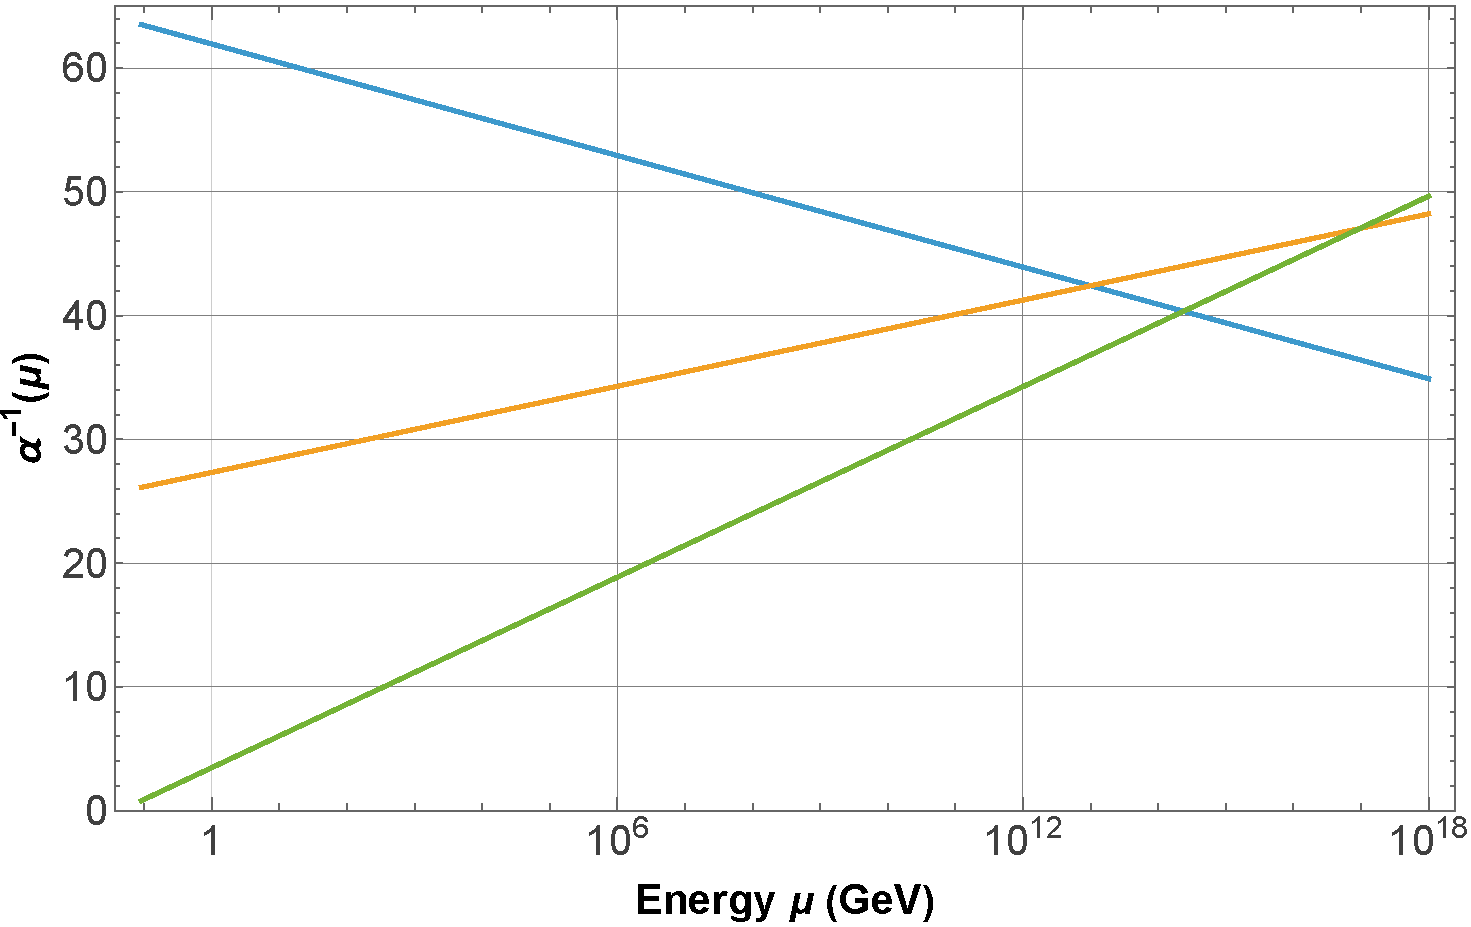
\includegraphics[width=0.8\textwidth]{Homework 7/p3.pdf}
    \caption{Sketch of $\alpha_i^{-1}(\mu)$ as a function of $\ln(\mu)$ from $M_Z$ up to $\mu\approx 10^{17}$ GeV.}
    \label{HW7:fig: Gauge coupling unification}
\end{figure}
First, we calculate their numerical values: 
\begin{align}
    \alpha_1^{-1}(\mu) &= 59 - \frac{41}{20\pi} \ln\left(\frac{\mu}{M_Z}\right) \\
    &= - \frac{41}{20\pi} \ln\left(\mu\right) + \frac{41}{20\pi} \ln\left(M_Z\right) + 59, \\
    \alpha_2^{-1}(\mu) &= 29.6 + \frac{19}{12\pi} \ln\left(\frac{\mu}{M_Z}\right) \\
    &= \frac{19}{12\pi} \ln\left(\mu\right) - \frac{19}{12\pi} \ln\left(M_Z\right) + 29.6, \\
    \alpha_3^{-1}(\mu) &= 8.5 + \frac{7}{2\pi} \ln\left(\frac{\mu}{M_Z}\right)\\
    &= \frac{7}{2\pi} \ln\left(\mu\right) - \frac{7}{2\pi} \ln\left(M_Z\right) + 8.5.
\end{align}
From the sketch in Fig.~\ref{HW7:fig: Gauge coupling unification}, we can see that the three couplings do not unify at a single scale in the Standard Model. The scale at which $\alpha_1$ and $\alpha_2$ meet is approximately $10^{13}$ GeV.

\begin{itemize}
    \item [(b)]
\end{itemize}

\begin{figure}[!th]
    \centering
    \begin{subfigure}{0.49\textwidth}
    \centering
    \begin{tikzpicture}
    \begin{feynman}
        % 外部粒子
        \vertex (i1) at (-2.5,2.5) {\(Q\)};
        \vertex (i2) at (-2.5,-2.5) {\(e_R^c\)};
        \vertex (f1) at (2.5,2.5) {\(Q\)};
        \vertex (f2) at (2.5,-2.5) {\(u_R^c\)};
        % 頂點
        \vertex (v1) at (-1,0);
        \vertex (v2) at (1,0);
        \diagram*{
            (i1)--[fermion, momentum={\(p_1\)}](v1) --[fermion, reversed momentum={\(p_2\)}](i2),
            (v1) --[photon, momentum'={\(\frac{-i}{q_s^2-M_X^2}\)},edge label={\(X_\mu\)}](v2),
            (f2)--[fermion, reversed momentum={\(p_3\)}](v2) --[fermion, momentum={\(p_4\)}] (f1),
        };  
        \node[left=5pt of v1] {\( i g_\text{GUT} \)};
        \node[right=5pt of v2]{\( i g_\text{GUT}\)};
    \end{feynman}
    \end{tikzpicture}
    \caption{Feynman diagram for $Q \overline{e_R^c} \to Q \overline{u_R^c}$ via s-channel scalar exchange. $q_s = p_1 + p_2 = p_3 + p_4$ is the momentum of the intermediate scalar.}
    \label{HW7:QQ-eu-scattering-s-channel}
    \end{subfigure}
    \begin{subfigure}{0.49\textwidth}
    \centering
    \begin{tikzpicture}
    \begin{feynman}
        % 外部粒子
        \vertex (i1) at (-2.5,2.5) {\(Q\)};
        \vertex (i2) at (-2.5,-2.5) {\(e_R^c\)};
        \vertex (f1) at (2.5,2.5) {\(Q\)};
        \vertex (f2) at (2.5,-2.5) {\(u_R^c\)};
        % 頂點
        \vertex (v1) at (-1,0);
        \vertex (v2) at (1,0);
        \vertex (v4point) at (0,0);
        \diagram*{
            (i1)--[fermion, momentum={\(p_1\)}](v4point) --[fermion, reversed momentum={\(p_2\)}](i2),
            (f2)--[fermion, reversed momentum={\(p_3\)}](v4point) --[fermion, momentum={\(p_4\)}] (f1),
        };  
        \node [left=5pt of v4point] {\(ig_\text{GUT}^2/M_X^2 \)};
    \end{feynman}
    \end{tikzpicture}
    \caption{Feynman diagram for $Q \overline{e_R^c} \to Q \overline{u_R^c}$ via a contact interaction. This diagram is obtained by integrating out the heavy $X$ boson in the s-channel diagram in Fig.~\ref{HW7:QQ-eu-scattering-s-channel}.}
    \label{HW7:QQ-eu-scattering-contact}
    \end{subfigure}
    \caption{Feynman diagrams for $Q \overline{e_R^c} \to Q \overline{u_R^c}$ scattering via gauge interactions.}
\end{figure}
The schematic couplings $g_\text{GUT} X_\mu Q^\dagger \overline{\sigma}^\mu e^c_R$ and $g_\text{GUT} X_\mu {u^c_R}^\dagger \overline{\sigma}^\mu Q$ are consistent with the Standard Model quantum numbers of the heavy gauge boson $X_\mu$. The first coupling describes the interaction between the heavy gauge boson $X_\mu$, the left-handed quark doublet $Q$, and the right-handed charged lepton $e_R^c$. The second coupling describes the interaction between the heavy gauge boson $X_\mu$, the right-handed up-type quark $u_R^c$, and the left-handed quark doublet $Q$. Integrating out the heavy $X$ boson of mass $M_X$ generates a low-energy dimension-6 operator of the form 
\begin{align}
    \mathcal{L}_\text{eff} \supset \frac{g_\text{GUT}^2}{M_X^2} (QQ) (e^c_R u^c_R),
\end{align}
up to contractions. 
\begin{figure}
    \centering
    \begin{tikzpicture}
    \begin{feynman}
        % 外部粒子
        \vertex (i1) at (-4,1) {\(u\)};
        \vertex (i2) at (-4,0) {\(u\)};
        \vertex (i3) at (-4,-1) {\(d\)};
        \vertex (f1) at (4,1) {\(e^+\)};
        \vertex (f2) at (4,-1) {\(\overline{d}\)};
        \vertex (f3) at (4,-1.5) {\(d\)};
        % 頂点
        \vertex (v1) at (0,1);
        \vertex (v2) at (0,0);
        \vertex (v4point) at (1,0.5);
        \vertex (v3) at (1,-1);
        \diagram*{
            (i1)--[fermion ](v1) --[fermion](v4point)--[fermion ](f1),
            (i2)--[fermion ](v2) --[fermion](v4point)--[fermion ](f2),
            (i3)--[fermion ](v3) --[fermion ](f3),
        };  
    \end{feynman}
    \end{tikzpicture}
    \caption{Feynman diagram for proton decay $p \to e^+ \pi^0$ mediated by the dimension-6 operator $(QQ)(e_R^c u_R^c)$. The initial state contains two up quarks and one down quark, which can be found inside the proton. The final state contains a positron $e^+$ and $d\overline{d}$ quark pair, which can hadronize into a $\pi^0$.}
    \label{HW7:fig:-Proton-decay}
\end{figure}
Figure~\ref{HW7:fig:-Proton-decay} shows a Feynman diagram for proton decay $p \to e^+ \pi^0$ via the dimension-6 operator $(QQ)(e_R^c u_R^c)$. This process is baryon-number violating because the initial state contains three quarks (baryon number $B=1$) while the final state contains no quarks (baryon number $B=0$). Hence, this operator can mediate proton decay. 

\begin{itemize}
    \item [(c)]
\end{itemize}
First, consider the dimension-6 operator $(QQ)(e_R^c u_R^c)$, which has a coefficient of $g_\text{GUT}^2/M_X^2$. The decay amplitude $\mathcal{M}$ for proton decay is proportional to this coefficient, so we have
\begin{align}
    \mathcal{M} \sim \frac{g_\text{GUT}^2}{M_X^2}.
\end{align}
The decay rate $\Gamma_p$ is proportional to the square of the amplitude, so we have
\begin{align}
    \Gamma_p \propto |\mathcal{M}|^2 \sim \frac{g_\text{GUT}^4}{M_X^4} \sim \alpha_\text{GUT}^2 \frac{1}{M_X^4}.
\end{align}
Since the decay rate is dimension of mass, we need to multiply by a factor of $M_p^5$ to get the correct dimensions, where $M_p$ is the proton mass. Hence, we have
\begin{align}
    \Gamma_p \sim \alpha_\text{GUT}^2 \frac{M_p^5}{M_X^4}.
\end{align}
The proton lifetime $\tau_p$ is the inverse of the decay rate, so we have
\begin{align}
    \tau_p \sim \frac{1}{\Gamma_p} \sim \frac{M_X^4}{\alpha_\text{GUT}^2 M_p^5}.
\end{align}
Now, we can estimate the proton lifetime for $M_X \approx 10^{15}$ GeV, taking $M_p = 1$ GeV and $\alpha_\text{GUT} \approx 1/25$. We have
\begin{align}
    \tau_p &\sim \frac{(10^{15} \text{ GeV})^4}{(1/25)^2 (1 \text{ GeV})^5} \\
    &= 25^2 \times 10^{60} \text{ GeV}^{-1} \\
    &\approx 6.25 \times 10^{62} \text{ GeV}^{-1}\\
    &\approx 6.25 \times 10^{62} \times 6.58 \times 10^{-25} \text{ s} \\
    &\approx 4.11 \times 10^{38} \text{ s} \\
    &\approx 1.30 \times 10^{31} \text{ years}.
\end{align}
This estimated proton lifetime is much shorter than the current lower limit $\tau(p\to e^+ \pi^0) \geq 10^{34}$ years, which means that if $M_X$ were around $10^{15}$ GeV, we would have already observed proton decay. 

Finally, we can use the scaling result to explain why the lower bound on $M_X$ depends only weakly on the experimental lower bound on the proton lifetime. Since $\tau_p \sim M_X^4$, we have
\begin{align}
    M_X \sim \tau_p^{1/4}.
\end{align}
This means that if the experimental lower bound on the proton lifetime increases by a factor of $10^n$, the lower bound on $M_X$ only increases by a factor of $10^{n/4}$. For example, if the lower bound on the proton lifetime increases from $10^{34}$ years to $10^{35}$ years (an increase by a factor of 10), the lower bound on $M_X$ only increases by a factor of $10^{1/4} \approx 1.78$. Specifically, to satisfy the current lower bound on the proton lifetime, we need
\begin{align}
    M_X &> 10^{15} \text{ GeV} \times 1.78^{(34-31)} \\
    &\approx 10^{15} \text{ GeV} \times 1.78^{3} \\
    &\approx 10^{15} \text{ GeV} \times 5.63 \\
    &\approx 5.63 \times 10^{15} \text{ GeV}.
\end{align}
\qed




